\documentclass[12pt, a4]{article}
\usepackage[english]{babel}
\usepackage[utf8x]{inputenc}
\usepackage{fullpage}
\usepackage{listings}
\usepackage{graphicx}
\usepackage{color}

%Syntax highlighting
\definecolor{blue-violet}{rgb}{0.54, 0.17, 0.89}
\definecolor{ao}{rgb}{0.0, 0.5, 0.0}
\definecolor{amaranth}{rgb}{0.9, 0.17, 0.31}
\definecolor{ballblue}{rgb}{0.13, 0.67, 0.8}
\definecolor{onyx}{rgb}{0.06, 0.06, 0.06}


\lstset{
  breaklines=true,                 % automatic line breaking only at whitespace
  captionpos=b,                    % sets the caption-position to bottom
  breakatwhitespace=false,
  keepspaces=true,
  numbers=left,
  numbersep=5pt,
  showspaces=false,
  showstringspaces=false,
  showtabs=false,
  tabsize=4,  
  backgroundcolor=\color{white},   % choose the background color
  commentstyle=\color{ao},    % comment style
  keywordstyle=\color{amaranth},    % keyword style
  stringstyle=\color{blue-violet},    % string literal style
  numberstyle=\tiny\color{ballblue},	   % number style
  basicstyle=\ttfamily\footnotesize\color{onyx} % size of fonts used for the code
}

%Document Header
\title{\textbf{Department of CSE\\SSN College of Engineering}}
\author{\textbf{Vishakan Subramanian - 18 5001 196 - Semester VII}}
\date{18 August 2021}

\begin{document}
\maketitle
\hrule
\section*{\center{UCS 1711 - Mobile Application Development Lab}}
\hrule
\bigskip

%Assignment Details
\subsection*{\center{\textbf{Exercise 3: Application Using Graphical Primitives}}}
\subsection*{\flushleft{Aim:}}
\begin{flushleft}
To develop an Android application that generates the following using graphical primitives.

\begin{enumerate}
\item Draw shapes such as Line, Circle, Rectangle and Arc.
\item Perform animations on an image.
\item Perform transformations like rotation and zoom.
\item Draw a car and animate the car.
\end{enumerate}

\end{flushleft}

%Code
\newpage
\subsection*{\flushleft{Code: Main Activity:}}
\begin{flushleft}
\lstinputlisting[language = Java]{Graphics/app/src/main/java/com/example/graphics/MainActivity.java}
\end{flushleft}

%Code
\newpage
\subsection*{\flushleft{Code: Shapes Activity:}}
\begin{flushleft}
\lstinputlisting[language = Java]{Graphics/app/src/main/java/com/example/graphics/ShapesActivity.java}
\end{flushleft}

%Code
\newpage
\subsection*{\flushleft{Code: Animate Activity:}}
\begin{flushleft}
\lstinputlisting[language = Java]{Graphics/app/src/main/java/com/example/graphics/AnimateActivity.java}
\end{flushleft}

%Code
\newpage
\subsection*{\flushleft{Code: Transform Activity:}}
\begin{flushleft}
\lstinputlisting[language = Java]{Graphics/app/src/main/java/com/example/graphics/TransformActivity.java}
\end{flushleft}

%Code
\newpage
\subsection*{\flushleft{Code: Rotate XML:}}
\begin{flushleft}
\lstinputlisting[language = XML]{Graphics/app/src/main/res/anim/rotate.xml}
\end{flushleft}

%Code
\newpage
\subsection*{\flushleft{Code: Fade XML:}}
\begin{flushleft}
\lstinputlisting[language = XML]{Graphics/app/src/main/res/anim/fade.xml}
\end{flushleft}

%Code
\newpage
\subsection*{\flushleft{Code: Zoom XML:}}
\begin{flushleft}
\lstinputlisting[language = XML]{Graphics/app/src/main/res/anim/zoom.xml}
\end{flushleft}

%Code
\newpage
\subsection*{\flushleft{Code: Main Activity Layout}}
\begin{flushleft}
\lstinputlisting[language = XML]{Graphics/app/src/main/res/layout/activity_main.xml}
\end{flushleft}

%Code
\newpage
\subsection*{\flushleft{Code: Shapes Activity Layout}}
\begin{flushleft}
\lstinputlisting[language = XML]{Graphics/app/src/main/res/layout/activity_shapes.xml}
\end{flushleft}

%Code
\newpage
\subsection*{\flushleft{Code: Animate Activity Layout}}
\begin{flushleft}
\lstinputlisting[language = XML]{Graphics/app/src/main/res/layout/activity_animate.xml}
\end{flushleft}

%Code
\newpage
\subsection*{\flushleft{Code: Transform Activity Layout}}
\begin{flushleft}
\lstinputlisting[language = XML]{Graphics/app/src/main/res/layout/activity_transform.xml}
\end{flushleft}


%Output
\newpage
\subsection*{\flushleft{Output: Graphics App Main Screen:}}
\begin{figure}[h]
\centering
\caption{Output: Graphics App Main Screen.}
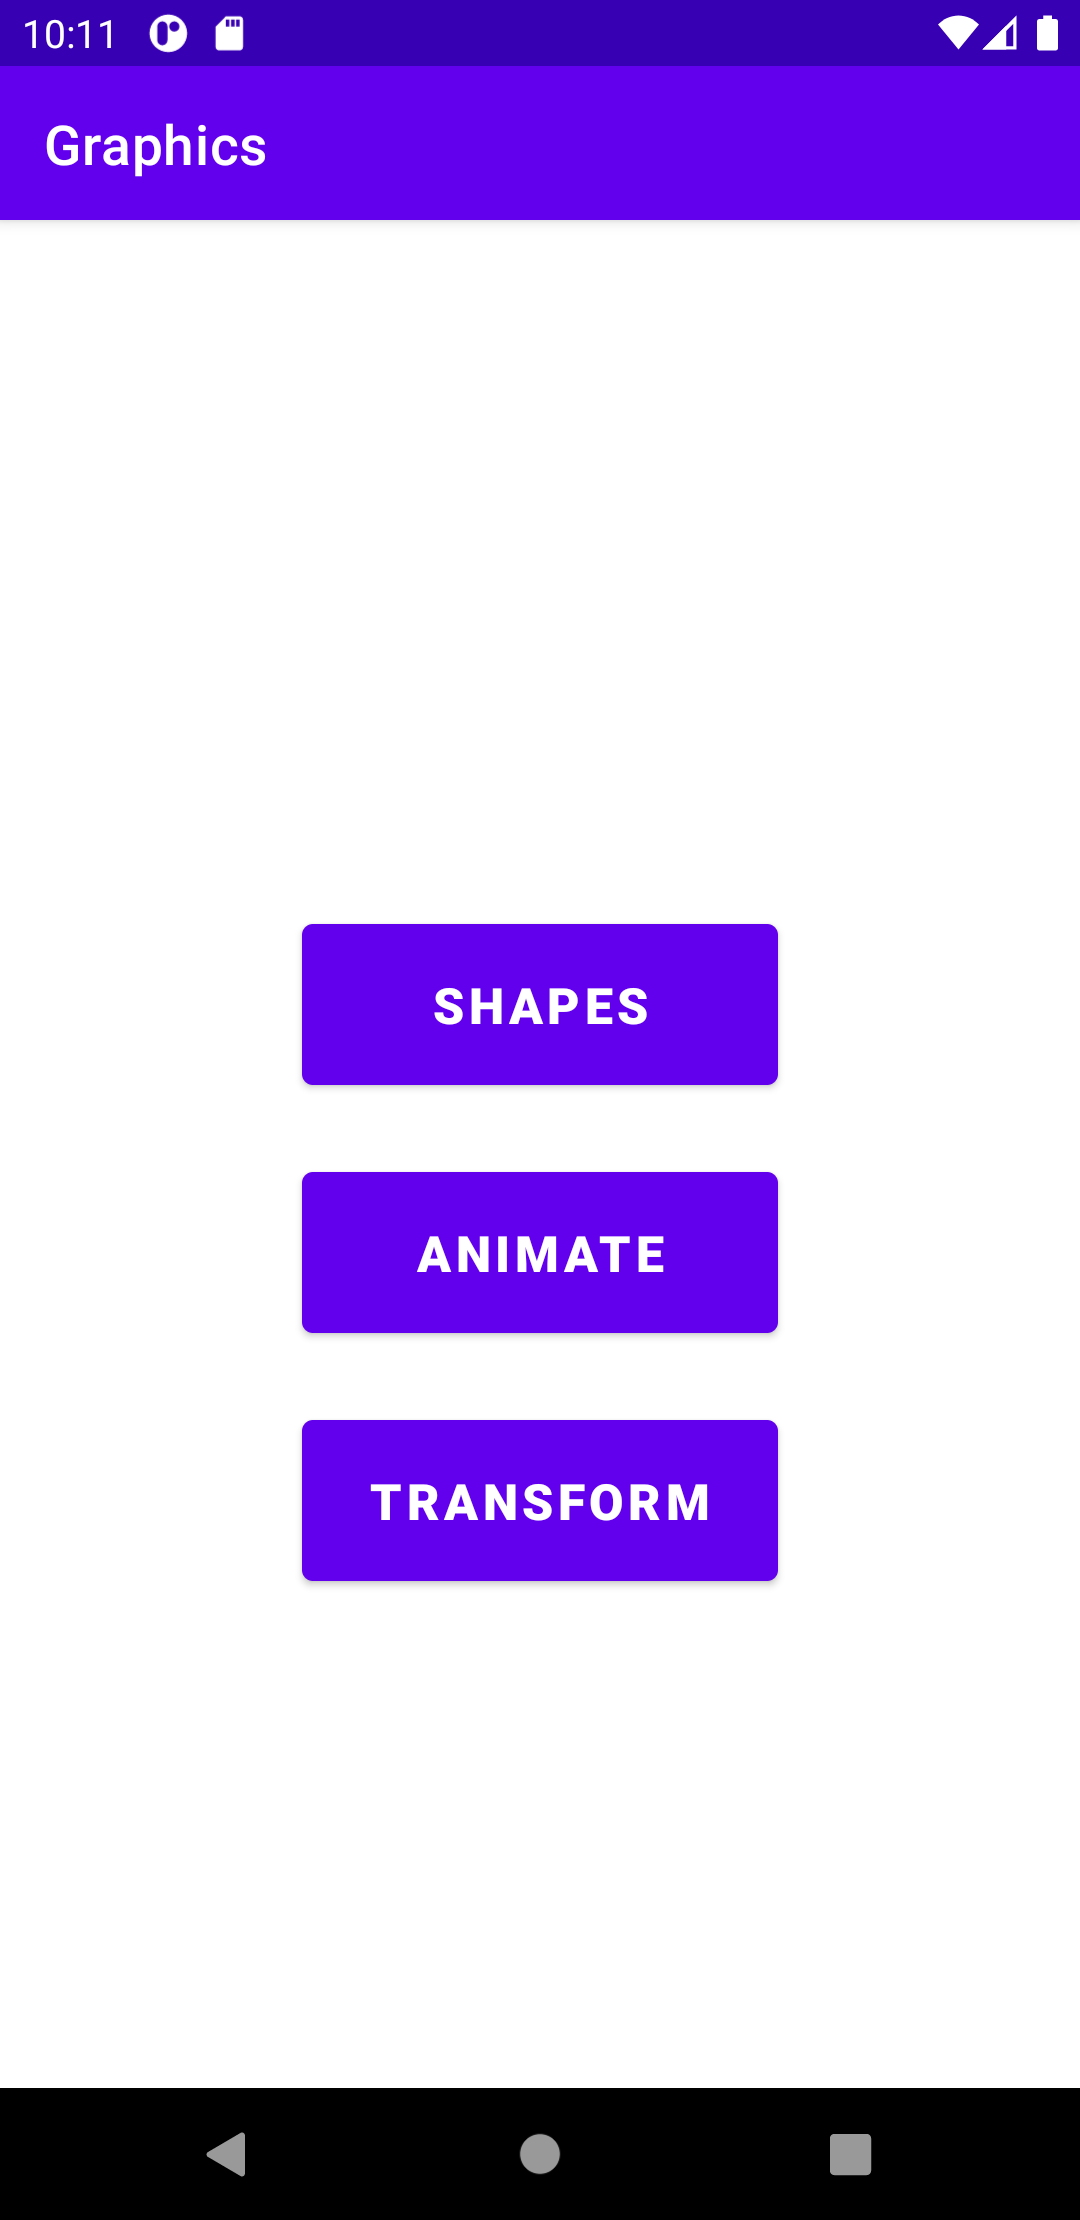
\includegraphics[height=15cm, width=7.3cm]{Graphics/Screenshots/Graphics-1.png}
\end{figure}

%Output
\newpage
\subsection*{\flushleft{Output: Shapes Screen:}}
\begin{figure}[h]
\centering
\caption{Output: Shapes Screen.}
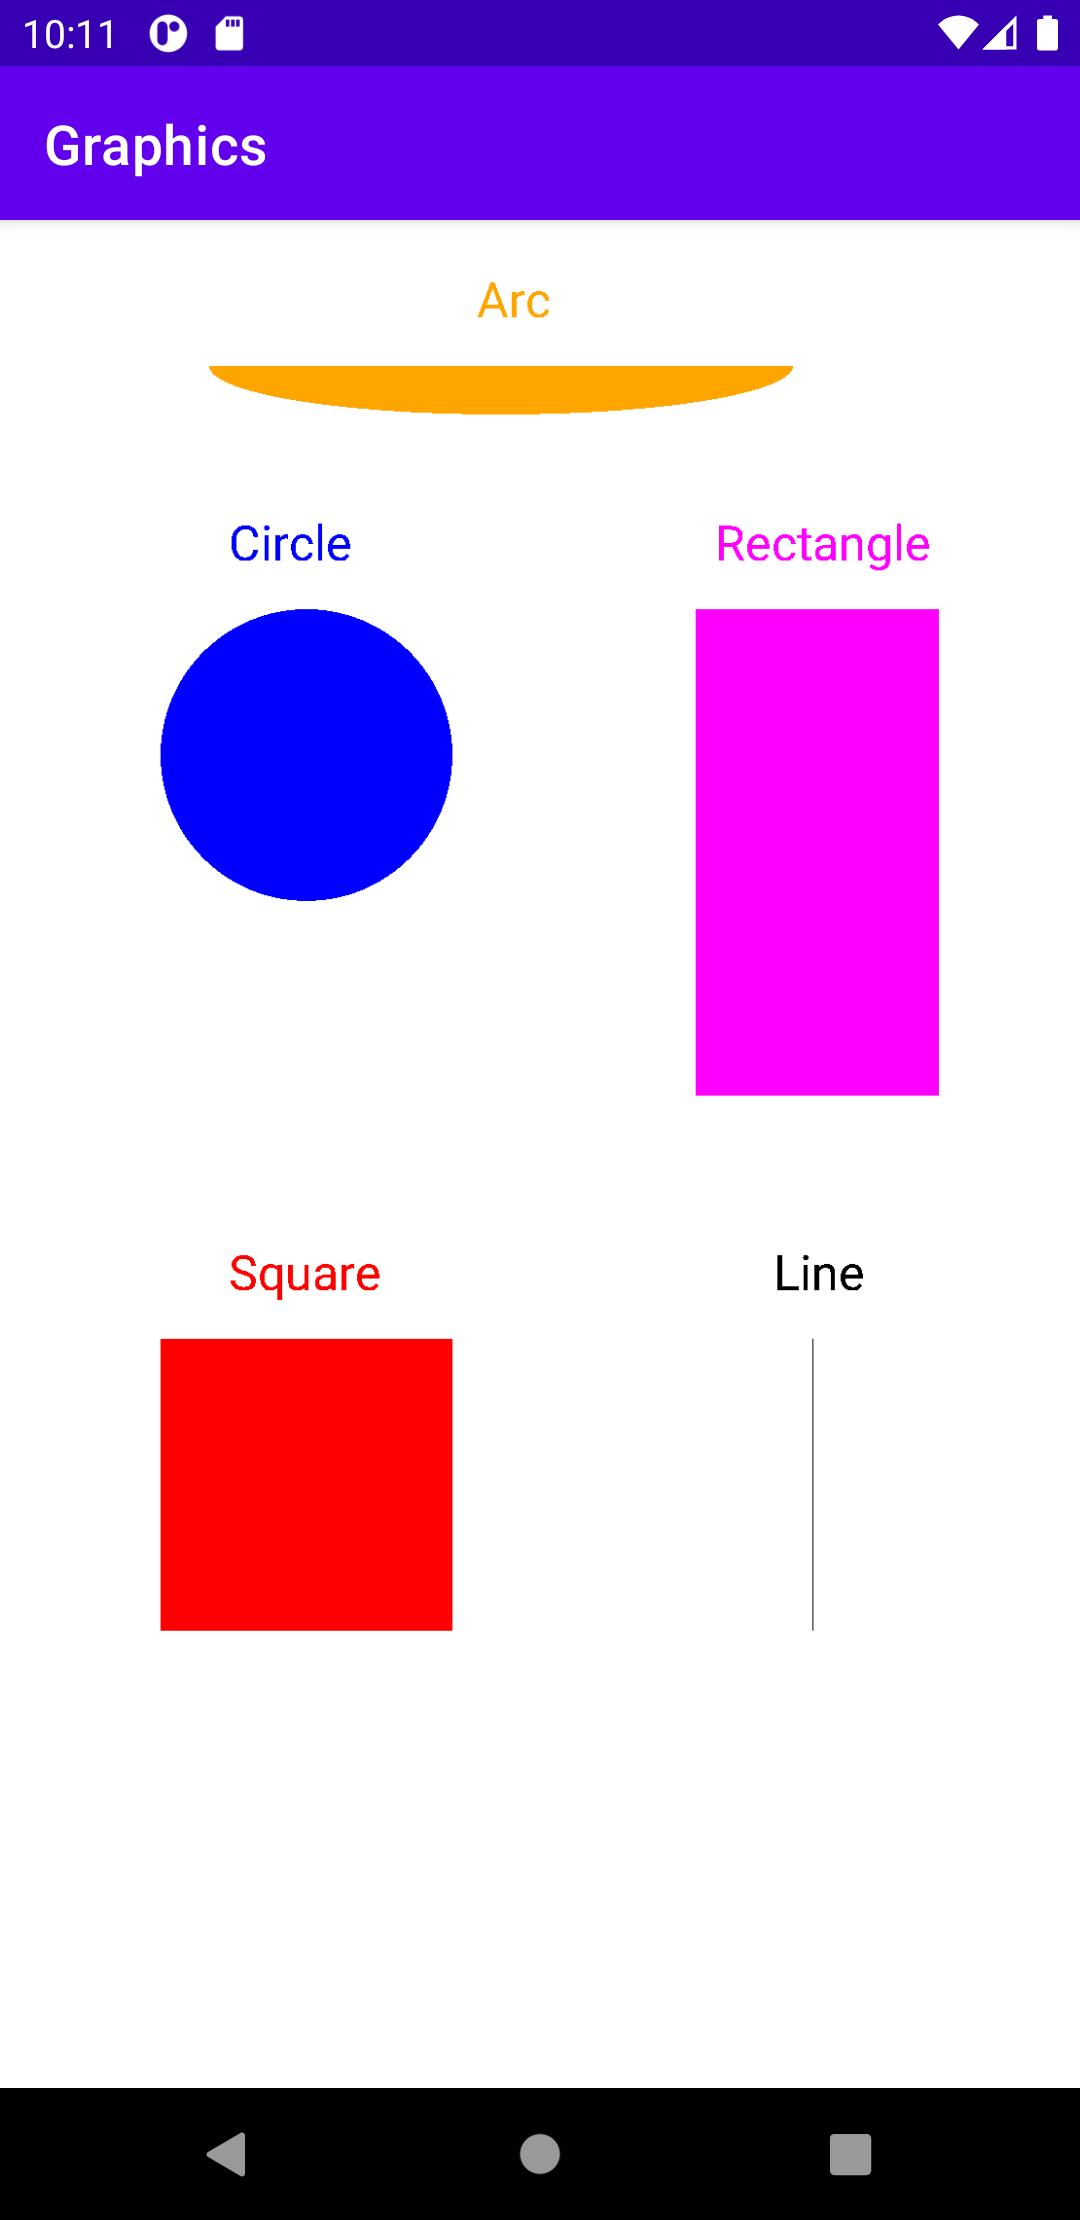
\includegraphics[height=15cm, width=7.3cm]{Graphics/Screenshots/Graphics-2.png}
\end{figure}

%Output
\newpage
\subsection*{\flushleft{Output: Animations Screen - 1:}}
\begin{figure}[h]
\centering
\caption{Output: Animations Screen - 1.}
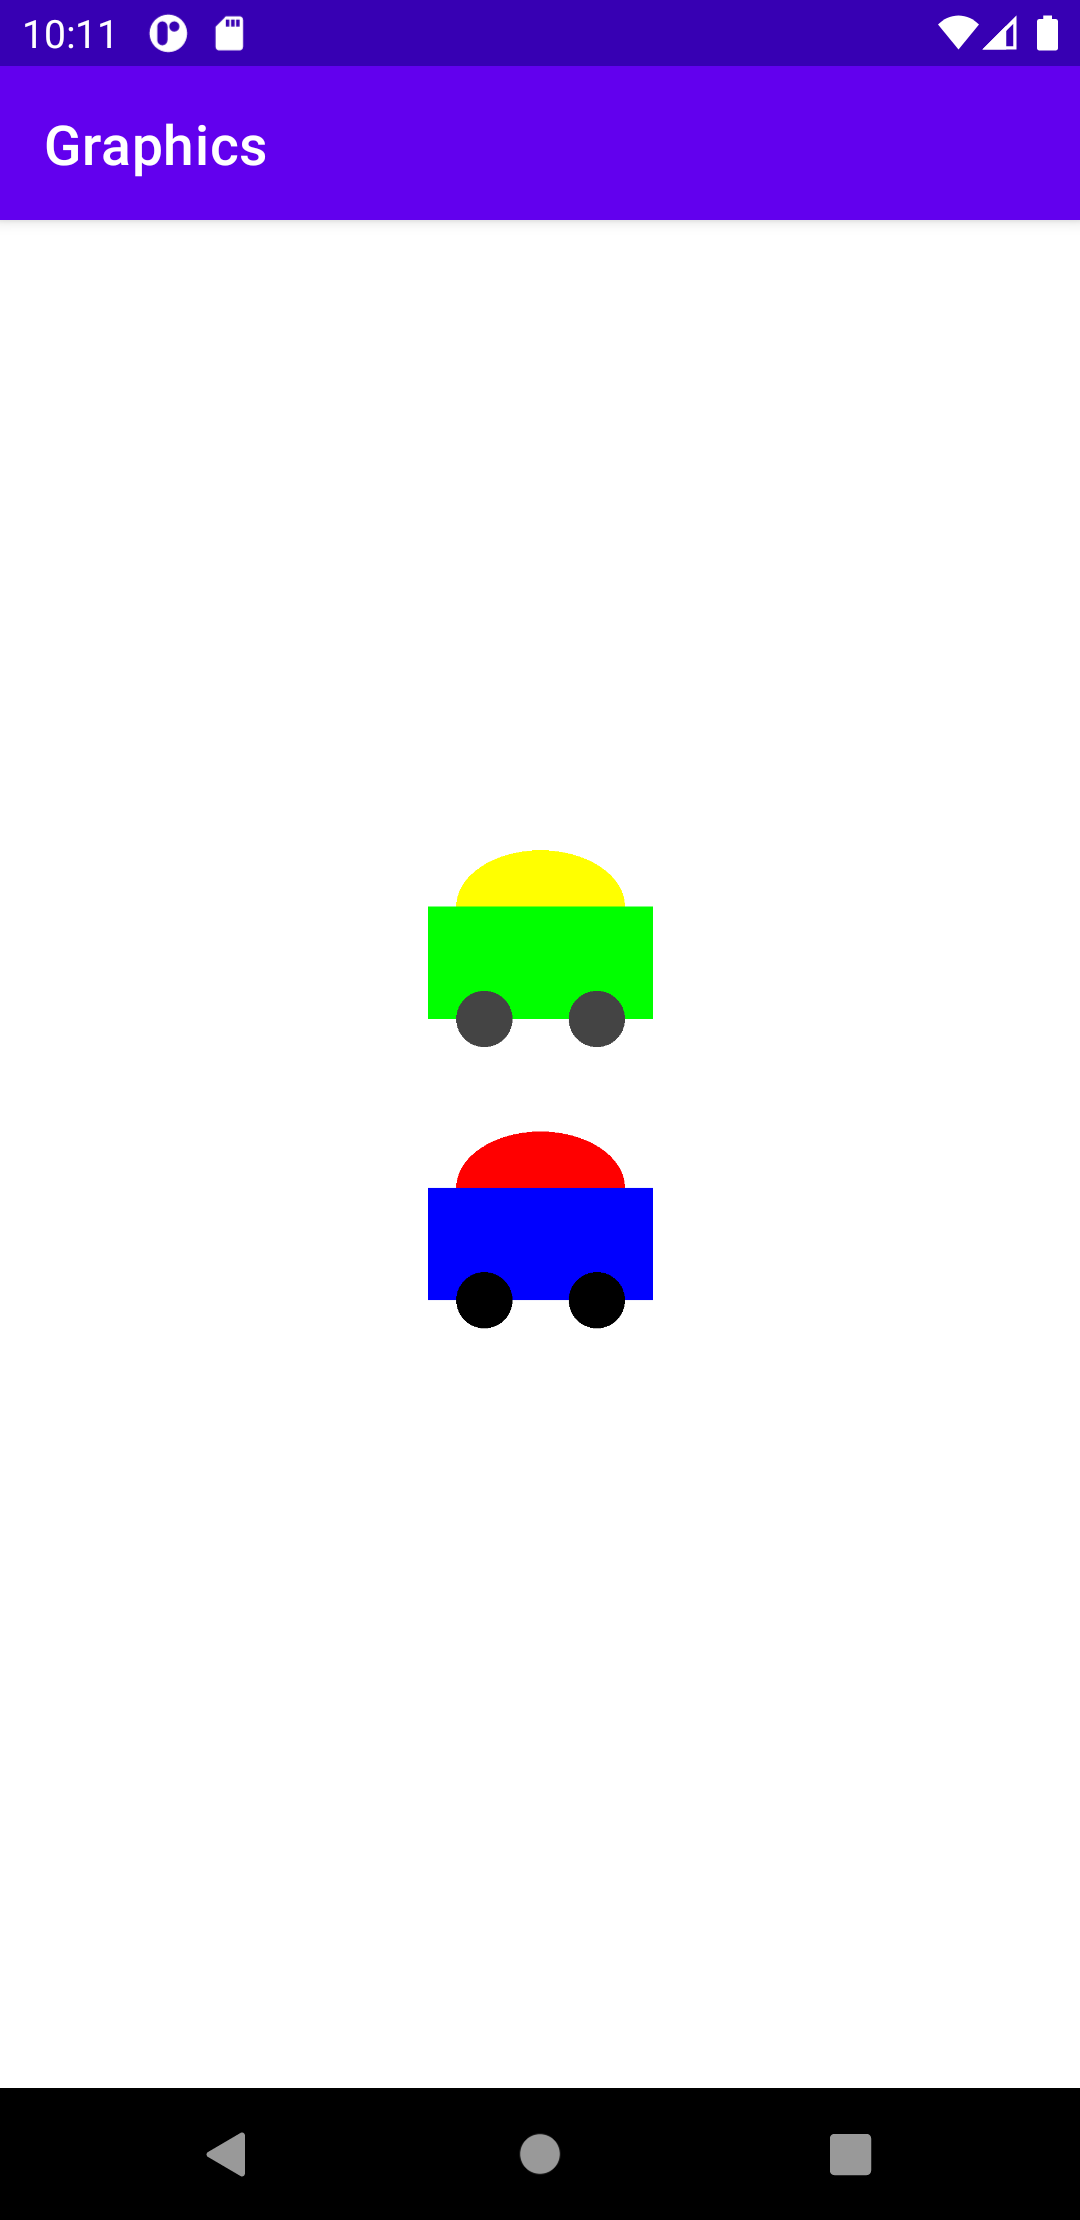
\includegraphics[height=15cm, width=7.3cm]{Graphics/Screenshots/Graphics-3.png}
\end{figure}

%Output
\newpage
\subsection*{\flushleft{Output: Animations Screen - 2:}}
\begin{figure}[h]
\centering
\caption{Output: Animations Screen - 2.}
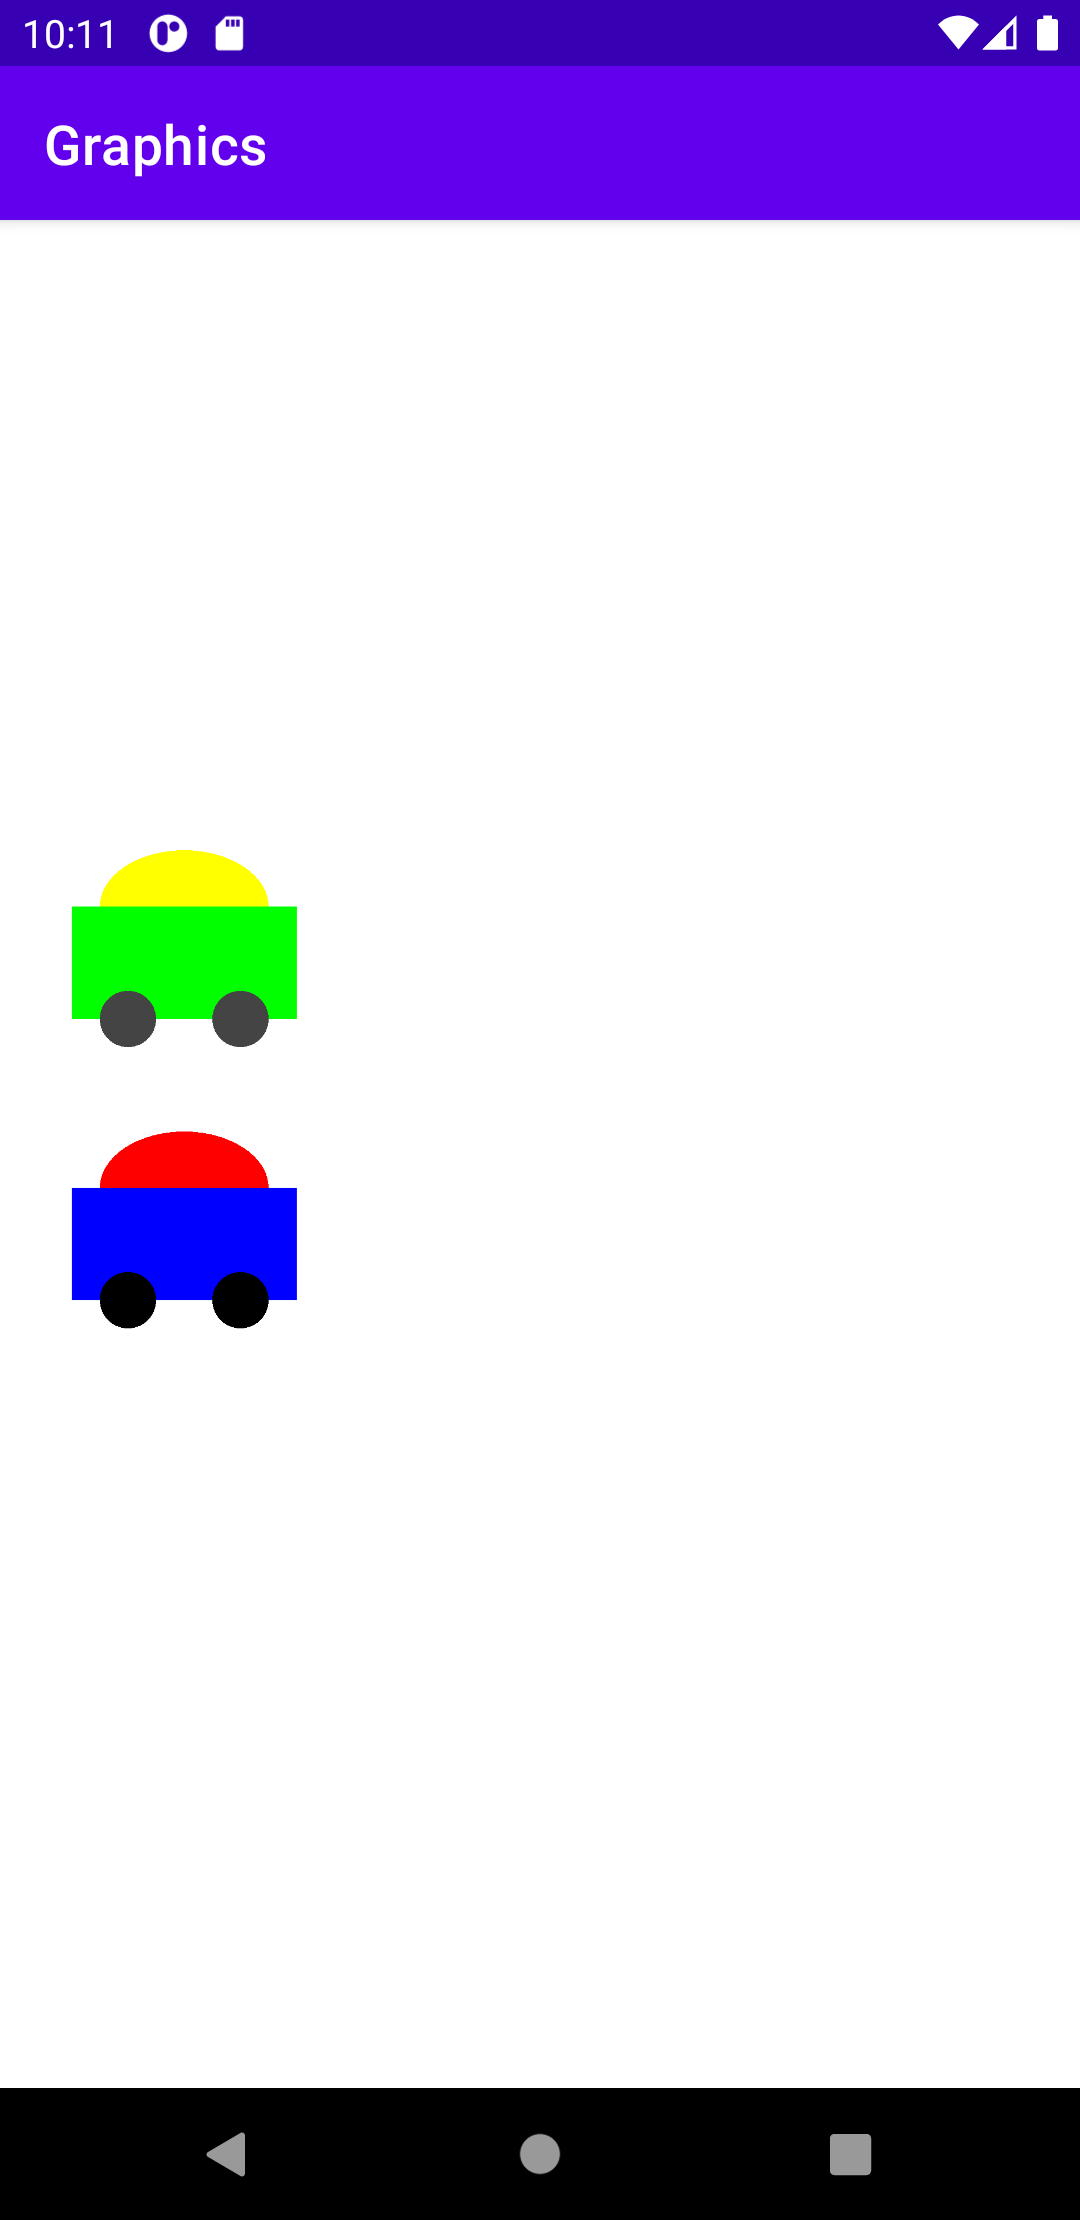
\includegraphics[height=15cm, width=7.3cm]{Graphics/Screenshots/Graphics-4.png}
\end{figure}

%Output
\newpage
\subsection*{\flushleft{Output: Transformations Screen - 1:}}
\begin{figure}[h]
\centering
\caption{Output: Transformations Screen - 1.}
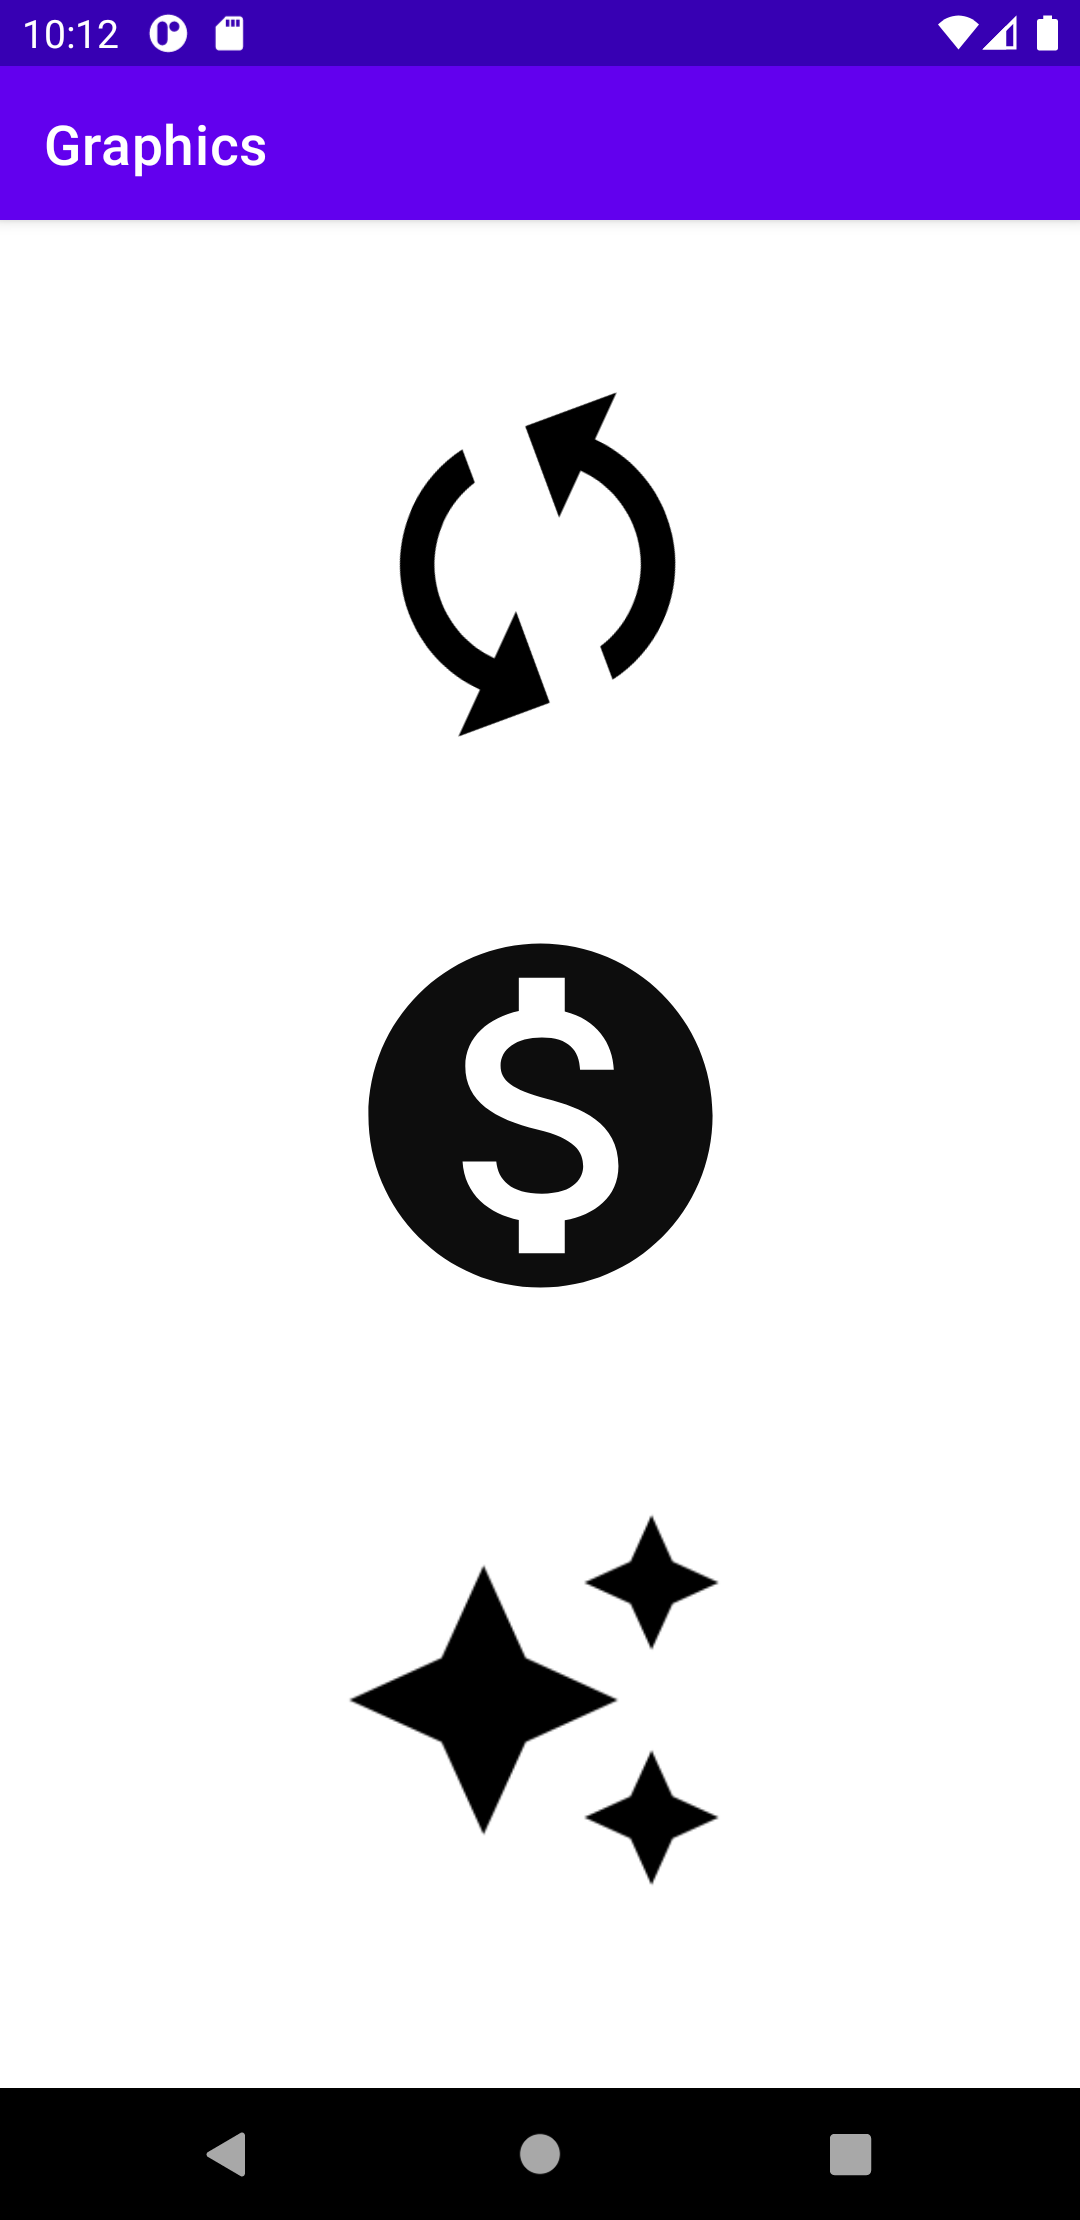
\includegraphics[height=15cm, width=7.3cm]{Graphics/Screenshots/Graphics-5.png}
\end{figure}

%Output
\newpage
\subsection*{\flushleft{Output: Transformations Screen - 2:}}
\begin{figure}[h]
\centering
\caption{Output: Transformations Screen - 2.}
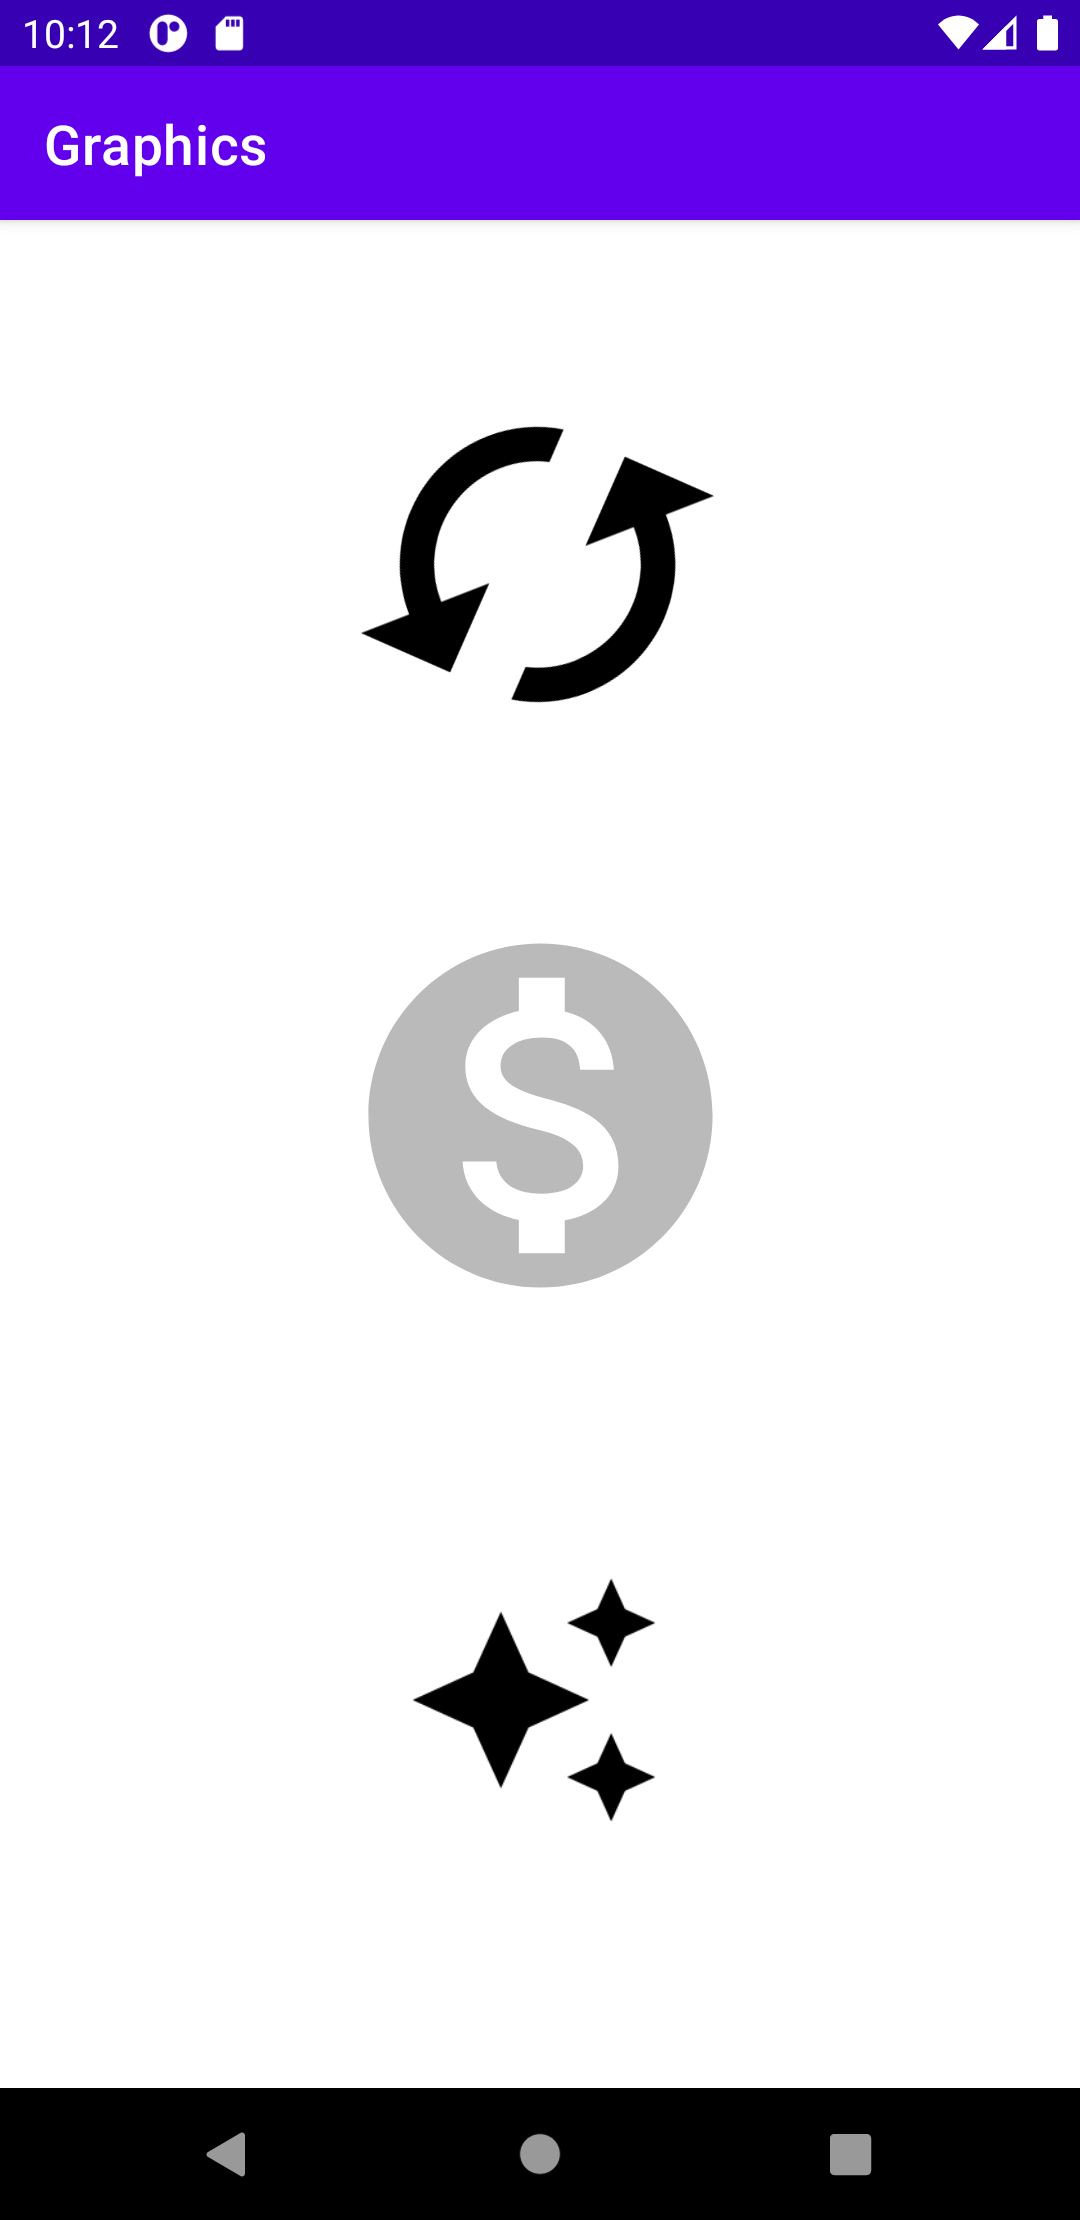
\includegraphics[height=15cm, width=7.3cm]{Graphics/Screenshots/Graphics-6.png}
\end{figure}


%Learning Outcome
\newpage
\subsection*{\flushleft{Learning Outcome:}}
\begin{itemize}
\item I understood how to draw graphical primitives like shapes using \textbf{Bitmap} and \textbf{Canvas} in Android.
\item I was able to draw shapes like \textbf{Lines, Rectangles, Circles and Arcs} using the Canvas object.
\item I was able to set \textbf{Colors} to the objects drawn using the Canvas object.
\item I drew a simple \textbf{car} using the graphical primitives.
\item I was able to animate the car to \textbf{move forwards and backwards} infinitely using \textbf{AnimatorSet} object.
\item I understood how to add custom animation specifications with XML-based syntax for Android applications.
\item I was able to add a \textbf{rotate} transformation to a static image using \textbf{AnimationUtils} object and \textbf{XML specification}.
\item I was able to add a \textbf{fade} transformation to a static image using \textbf{AnimationUtils} object and \textbf{XML specification}.
\item I was able to add a \textbf{zoom} transformation to a static image using \textbf{AnimationUtils} object and \textbf{XML specification}.
\item I understood how to use several XML-based parameters like \textbf{duration, repeatCount, repeatMode, pivotX, pivotY, fromXScale, fromYScale etc.} to control the transformations as desired.
\end{itemize}


\end{document}